\chapter{Experimental work} % Main chapter title
\label{Chapter2} % Change X to a consecutive number; for referencing this chapter elsewhere, use \ref{ChapterX}

%----------------------------------------------------------------------------------------
%	SECTION 1
%----------------------------------------------------------------------------------------
\subsection{Grips linked to hydraulic press}

To determine the load speed, the frequency of the camera recording and others experimental parameters, it was important to read previous works on the subject and determine which engines will be used to proceed the experiments. The hydraulic press used to pull on each side of the specimen is shown on \ref{fig:Fig8_a}

It is used in addition with the presented grips \ref{fig:Fig8_b}. These ones, si
\parencite{Reference17} works allow to find how the load must be applied. Indeed, it gives an approximation of loads values or displacement speed. The load speed recommended is about 0,1mm/min according to these texts. \parencite{Reference7} used the same loading speed around 5mm/min. The records are made at a frequency of 5Hz, so 5 images per second, according to \parencite{Reference17} or \parencite{Reference16}.
\parencite{Reference7} works helps to specify this type of parameters on MMCG samples. It is obvious that there are many similituds with DCB works. Indeed MMCG geometry is an adaptation of DCB and CTS ones, that explain why many parameters are the same.

%----------------------------------------------------------------------------------------
%	SUBSECTION 2
%----------------------------------------------------------------------------------------
\subsection{Hydraulic press setup}

The Hydraulic press, was setup by Mr Martins. The first step was to asssembled the grips in the press. They are screwed, for the first one, into one static part of the press, the upper side. The other grip is placed in the moving part. Between every tests, the grips must be desassembled and well scrwed to maintain each specimen, as well as possible. To change the specimen between two tests, manual command are used to elevate the moving part of the press and avoid the tension in the grips.
Then a displacement of 0.033mm/s was input in the press controler program. A 10kN load was also input to be sure that the displacement will occure correctly. Then the same load was applied but from the third specimen tested, a displacement of 0.015mm/s was finally applied. The position and the load is given at each time by the MTS software controler. Moreover, a plot is created in real time.

It was important to stop the press if too much tests are done, in order to avoid the overheating of the oil/water allimenting the hydraulic press. Indeed, it could involves problems as a quick raise or fall of the moving part of the press, destroying a specimen without capturing any images. This is why it is important to alway have someone near the urgent button on the manual control panel.

%----------------------------------------------------------------------------------------
%	SECTION 2
%----------------------------------------------------------------------------------------


%%%%%%%%%%%%%%%%%%%%%%%%%%%%%%%%%%%%%%%%%%%%%%%%%%%%%%%%%%

As it is visible, the average moisture content is around 9.20\% for Okoume specimens and 6.10\% for Padouck specimens. There are only three specimens of Iroko, which does not allow a efficient average, but it is around 7,5\% MC. It is important to notice that the specimen were dried and wait almost 24 hours before being weighed. That involves potential mistakes in the moisture content values calculated on the dried weight.
\section{Used Engines and material}

To determine the load speed, the frequency of the camera recording and others experimental parameters, it was important to read previous works on the subject and determine which engines will be used to proceed the experiments. The hydraulic press used to pull on each side of the specimen is shown on \ref{fig:Fig8_a}

\begin{figure}[th]
	\centering
	\begin{subfigure}{0.48\linewidth}
		\includegraphics[scale=0.034,angle=-90]{Figures/MSC_press}
		\decoRule
		\caption[MTS hydraulic press]{MTS hydraulic press, model 661.21B-03 allowing a maximal applied load of 10 metric to N}
		\label{fig:Fig8_a}
	\end{subfigure}
	\hfill
	\begin{subfigure}{0.48\linewidth}
		\includegraphics[scale=0.04]{Figures/Grips}
		\decoRule
		\caption[Grips]{Grips used to connect the MTS press and the spcimen.}
		\label{fig:Fig8_b}
	\end{subfigure}
	\caption{Experiment engine components}
	\label{fig:Fig8}
\end{figure}
It is used in addition with the presented grips \ref{fig:Fig8_b}. These ones, simpler than ARCAN system, allow to do mode I experiments. They were designed specially for MMCG dimensions near Caparica campus. The system is composed of a main piece which can be added in the mechanical press.Then, a pin allows to place two connectors from each side of the MMCG specimen. Finally, another pin goes through the connectors and the specimen holes.
\parencite{Reference17} works allow to find how the load must be applied. Indeed, it gives an approximation of loads values or displacement speed. The load speed recommended is about 0,1mm/min according to these texts. \parencite{Reference7} used the same loading speed around 5mm/min. The records are made at a frequency of 5Hz, so 5 images per second, according to \parencite{Reference17} or \parencite{Reference16}.
\parencite{Reference7} works helps to specify this type of parameters on MMCG samples. It is obvious that there are many similituds with DCB works. Indeed MMCG geometry is an adaptation of DCB and CTS ones, that explain why many parameters are the same.

%----------------------------------------------------------------------------------------
%	SECTION 2
%----------------------------------------------------------------------------------------
\section{Specimen preparation}

To begin with, all the specimens were named as presented in \ref{tab:Tab3}. It helps, to follow the evolution of each sample.
In this document, these names will be used. Their composition are made of the number of the experiment :
\newline
E1 : Test at an ambiant temperature and an ambiant MC
\newline
E2 : Test at an ambiant temperature and specimens with 30\% MC
\newline
E3 : Test at an ambiant temperature and specimens with 20\% MC
\newline
E4 : Test at a cooler temperature
\newline
E5 : Test at a hotter temperature
\newline
F : Test with Fatigue loads
\newline
Pbis/Pter : are 2 others specimens which were used to calibrate the tests
\newline
\newline
Then the name as a second component, which is the specie and the number of the specimen of this specie dedicated to this test.
\newline
O : Okoume
\newline
P : Padouck
\newline
I: Iroko
\newline
\newline
Finally, all the specimens are named like E1O1 which is the first specimen of Okoume used for the first type of experiment (ambient temperature and MC due to relative humidity in the air). These names were first written on specimens, but they disapeared when the specimens were put into water. So finally, names were engraved with a cutter. %indicate in case a problem occures due to the missing material

The 30 specimens bring from Polytech laboratory was weighed as soon as the sanitary condition (Covid pandemic) allows to do it. The scale used to weight the specimen was really precise, it is the GR-200 which is a Semi-Micro Analytical Balances. This precision is also made by the subtraction of air in the glass box, allowing a precision with the thousandths gramme as visible on \ref{fig:Fig9}. Its capacity can not reach 210g which does not affect the measures with a max weight of the denser wood, the Padouck, around 70.5g and a minimum weight of Okoume specimens with a weight of 36g
\begin{figure}[th]
	\centering
	\includegraphics[scale=0.05,angle=-90]{Figures/Balance_Test}
	\decoRule
	\caption[GR-200 Scale]{GR-200 Scale weigthing an Okoume specimen}
	\label{fig:Fig9}
\end{figure}

After this analyse, weight values were inputed in an Excel file. A resume is presented below in \ref{tab:Tab1} but the entire one is \ref{tab:Tab3}

\begin {table}[h]
\centering
\begin{tabular}{|c|r|}
	\hline
	\cellcolor[rgb]{ .973,  .796,  .678}
	okoume average weight &
	\cellcolor[rgb]{ 1,  1,  1}
	40,55 g \\
	\hline
	\cellcolor[rgb]{ .776,  .349,  .067}
	padouck average weight &
	\cellcolor[rgb]{ 1,  1,  1}
	66,29 g \\
	\hline
	\cellcolor[rgb]{ .749,  .561,  0}
	iroko average weight &
	\cellcolor[rgb]{ 1,  1,  1}
	54,33 g
\end{tabular}
\caption[specimens average weight]{specimens average weight depending on the species}
\label{tab:Tab1}
\end{table}
The next step was to dry them. The oven was not available at the faculty, so Mr Rui Martins dry the specimen during 24h at 103\textcelsius. The scale was not the same and some specimens were weighed again before the drying process to obtain an uncertainty. The uncertainty was applied on every specimen and written in the Excel file. The purpose was to determine the potential difference of the weight between the specimen weight at the faculty and the one by Rui Martins. Then the drying experiment gives the $M_{0}$ weight of the samples. $M_{0}$ as explained is the dried weight of a sample in gramme. It is used to calculate the moisture content in the sample. So, a new column was filled in the table \label{tab:Tab3} with the ambient moisture content. All the results are shown below, linked to the formula \ref{eq:Moisture content depending on weight}, given in previous chapters.

%MEttre en annexe le tableau final !

%\begin{figure}[h]
%	\centering
%	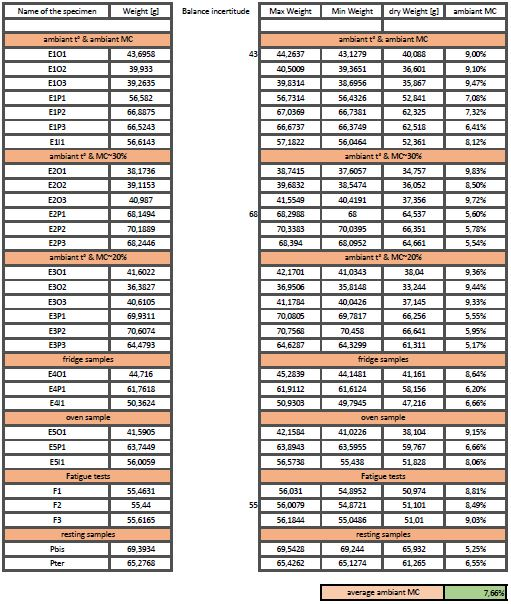
\includegraphics[width=\textwidth]{Figures/Specimen weight}
%	\decoRule
%	\caption[Specimen weight]{Table with weight values of each specimen}
%	\label{fig:Fig10}
%\end{figure}

As it is visible, the average moisture content is around 9.20\% for Okoume specimens and 6.10\% for Padouck specimens. There are only three specimens of Iroko, which does not allow a efficient average, but it is around 7,5\% MC. It is important to notice that the specimen were dried and wait almost 24 hours before being weighed. That involves potential mistakes in the moisture content values calculated on the dried weight.

Then, notches were created in each specimen. A precrack is made by a cutter into the notch. The interest is to initiate a straight crack, thanks to this first one.
%%%%%%%%%%%%%%%%%%%%%
The next step was to dry them. The oven was not available at the faculty, so Mr

As it is visible, the average moisture content is around 9.20\% for Okoume specimens and 6.10\% for Padouck specimens. There are only three specimens of Iroko, which does not allow a efficient average, but it is around 7,5\% MC. It is important to notice that the specimen were dried and wait almost 24 hours before being weighed. That involves potential mistakes in the moisture content values calculated on the dried weight.

Then, notches were created in each specimen. A precrack is made by a cutter into the notch. The interest is to initiate a straight crack, thanks to this first one. The notch width is around 1.5mm, done by a straight electrical saw : the Dexter Power NC500JS, and a blade of 1.27mm. Then the cutter allow to go deeper and creat a precrack with a shape allowing the propagation of the crack. As the denser one, Padouck was the most difficult wood in which these operation was done. the electrical saw involved smoke and a burnt smell, then cutter precrack was not as uniform as desired. \ref{tab:Tab11} show all the dimensions of this precrack.
\begin{table}[]
	\centering
	\begin{tabular}{c|c|}
		\cline{2-2}
		\multicolumn{1}{l|}{} & \multicolumn{1}{l|}{initial crack length} \\ \hline
		\multicolumn{1}{|c|}{\cellcolor[HTML]{F8CBAD}E1O1} & 26,5 mm \\ \hline
		\multicolumn{1}{|c|}{\cellcolor[HTML]{F8CBAD}E1O2} & 26,5 mm \\ \hline
		\multicolumn{1}{|c|}{\cellcolor[HTML]{F8CBAD}E1O3} & 25 mm \\ \hline
		\multicolumn{1}{|c|}{\cellcolor[HTML]{C65911}E1P1} & 25,5 mm \\ \hline
		\multicolumn{1}{|c|}{\cellcolor[HTML]{C65911}E1P2} & 25 mm \\ \hline
		\multicolumn{1}{|c|}{\cellcolor[HTML]{C65911}E1P3} & 25,5 mm \\ \hline
		\multicolumn{1}{|c|}{\cellcolor[HTML]{BF8F00}E1I1} & 26,5 mm \\ \hline
		\multicolumn{1}{|c|}{\cellcolor[HTML]{F8CBAD}E2O1} &  \\ \hline
		\multicolumn{1}{|c|}{\cellcolor[HTML]{F8CBAD}E2O2} &  \\ \hline
		\multicolumn{1}{|c|}{\cellcolor[HTML]{F8CBAD}E2O3} &  \\ \hline
		\multicolumn{1}{|c|}{\cellcolor[HTML]{C65911}E2P1} &  \\ \hline
		\multicolumn{1}{|c|}{\cellcolor[HTML]{C65911}E2P2} &  \\ \hline
		\multicolumn{1}{|c|}{\cellcolor[HTML]{C65911}E2P3} &  \\ \hline
		\multicolumn{1}{|c|}{\cellcolor[HTML]{F8CBAD}E3O1} &  \\ \hline
		\multicolumn{1}{|c|}{\cellcolor[HTML]{F8CBAD}E3O2} &  \\ \hline
		\multicolumn{1}{|c|}{\cellcolor[HTML]{F8CBAD}E3O3} &  \\ \hline
		\multicolumn{1}{|c|}{\cellcolor[HTML]{C65911}E3P1} &  \\ \hline
		\multicolumn{1}{|c|}{\cellcolor[HTML]{C65911}E3P2} &  \\ \hline
		\multicolumn{1}{|c|}{\cellcolor[HTML]{C65911}E3P3} &  \\ \hline
		\multicolumn{1}{|c|}{\cellcolor[HTML]{F8CBAD}E4O1} & 25,5 mm \\ \hline
		\multicolumn{1}{|c|}{\cellcolor[HTML]{C65911}E4P1} & 25,5 mm \\ \hline
		\multicolumn{1}{|c|}{\cellcolor[HTML]{BF8F00}E4I1} & 25,5 mm \\ \hline
		\multicolumn{1}{|c|}{\cellcolor[HTML]{F8CBAD}E5O1} & 27 mm \\ \hline
		\multicolumn{1}{|c|}{\cellcolor[HTML]{C65911}E5P1} & 24 mm \\ \hline
		\multicolumn{1}{|c|}{\cellcolor[HTML]{BF8F00}E5I1} & 25,5 mm \\ \hline
		\multicolumn{1}{|c|}{\cellcolor[HTML]{C65911}Pbis} & 25,5 mm \\ \hline
		\multicolumn{1}{|c|}{\cellcolor[HTML]{C65911}Pter} & 25,5 mm \\ \hline
	\end{tabular}
	\caption{Precrack dimensions}
	\label{tab:Tab11}
\end{table}
All the specimens were weighed again, due to the material taken away by the creation of the notch.
Specimens were weighed two times, to find the real difference between the scale from the laboratory and those of Mr Martins. A difference around 0.6g was found. Finally, specimens were put into water as it is visible on \ref{fig:Fig13}
\begin{figure}[h]
	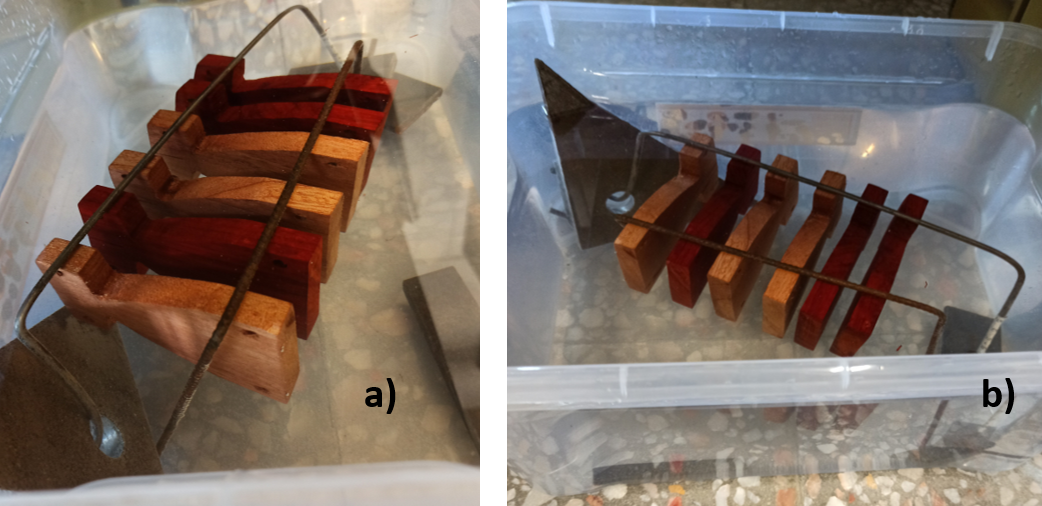
\includegraphics[width=\textwidth]{Figures/WaterSpecimens}
	Specimens were weighed two times, to find the real difference between the scale
\end{figure}
The system was designed in order to prevent the specimens from rising to the surface by flotation. But also, to minimize the specimen surface in contact with the system. Indeed, it allows to maximize the MC rise which take less time to reach the desired MC levels. This fact was verified when all the specimens (from E2 and E3 experiment) were put together into water. Indeed, the system was not designed for 12 specimens, and the specimens were really closed. It involves a slower increase of the MC.

After 80.62h, specimens were weighed again. Thanks to these weights, it was possible to plot a shape about, how the MC decreases, and how the weight evolve compared to time. A quick look to the decrease of MC into Okoume specimens show that until 20\% MC, every hour almost 1\% MC is loose. From this value until the ambient MC, the MC decrease process becomes slower as it is shown on \ref{fig:Fig15_b}, with decreasment less than 0.4\% every hour.

Thanks to E3 daily weight, it appears that both species, Okoume and Padouck, earn a constant MC. The difference is the value of this constant increasing. Okoume specimens earn approximately 5\% MC each day while Padouck ones earn around 2\% MC.

But wood is a living material with a really particular behavior. Looking to this previous parameters, visible in \ref{fig:Fig15_a} and \ref{fig:Fig15_b} an approximation was made. By puting out of the water the specimens at a given hour, they will be tested at a given other. By processing this way, a lot of the experiments were scedulled for 53h after puting them off the water. But in 7 hours Okoume specimen loose around 20\% of MC and Padouck around 7\%. Which is following the previous curve but for Padouck specimen it was quicker than expected.

\subsection{Specimens experimental setup}

To test the specimens at the waited MC, plots as the \ref{fig:Fig15_a} were used. Indeed, by looking to there weight when they were out the water, a MC was obtained, and by looking to the difference between the current MC and the waited one can be given in term of hours. So it was possible to have an approximation of the time before doing the experiments.

All the specimens were painted to obtain a patern which allows a treatment of the images. Indeeed it will be necessary for MatchID to have speckles composed of a given number of pixels. A white first layer was added and a black point cloud was a second painting layer. All the paint used are mate ones and not brilliant ones.
\begin{figure}[th]
	\centering
	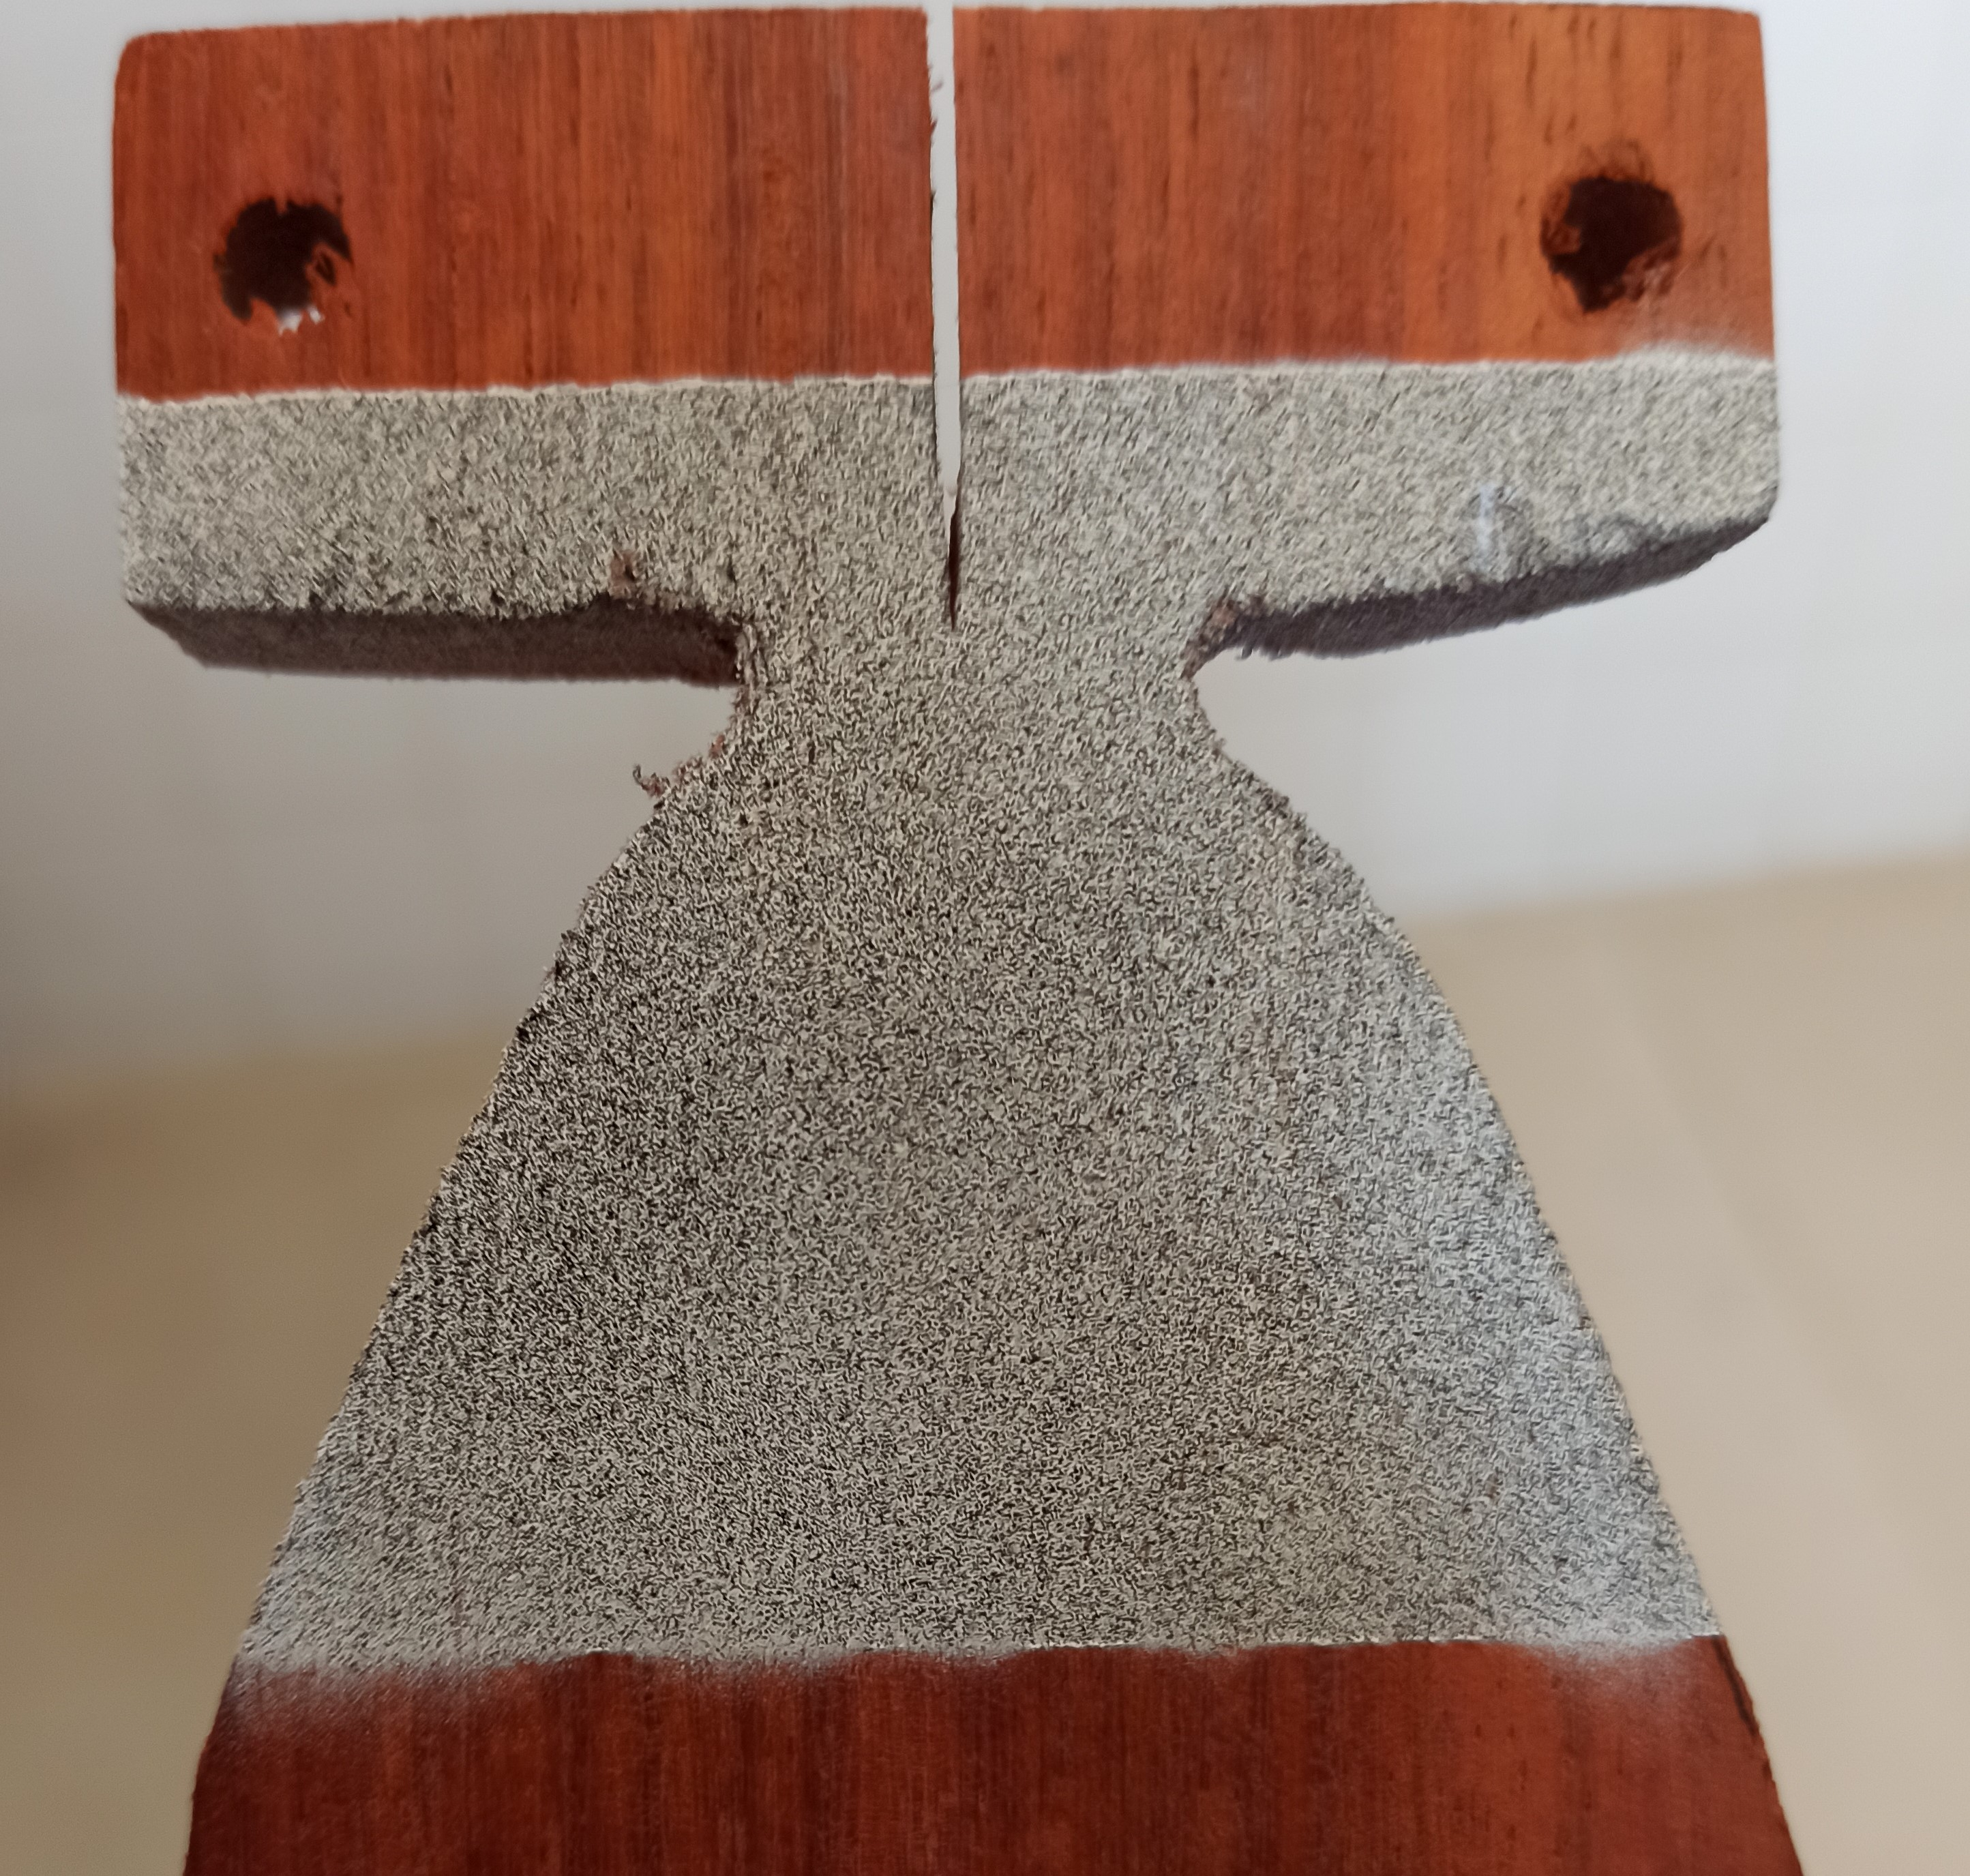
\includegraphics[scale=0.08]{Figures/Painted_specimen}
	All the specimens were painted to obtain a patern which allows a treatment of th
	\caption[Padouck painted specimen]{Padouck painted specimen before experimental test}
	\label{fig:Fig17}
\end{figure}

%%%%%%%%%%%%%%%%%%%%%%%%
The notch width is around 1.5mm, done by a straight electrical saw : the Dexter Power NC500JS, and a blade of 1.27mm. All the specimens were weighed again, due to the material taken away by the creation of the notch.
Specimens were weighed two times, to find the real difference between the scale from the laboratory and those of Mr Martins. A difference around 0.6g was found. Finally, specimens were put into water as it is visible on \ref{fig:Fig13}
\begin{figure}[h]
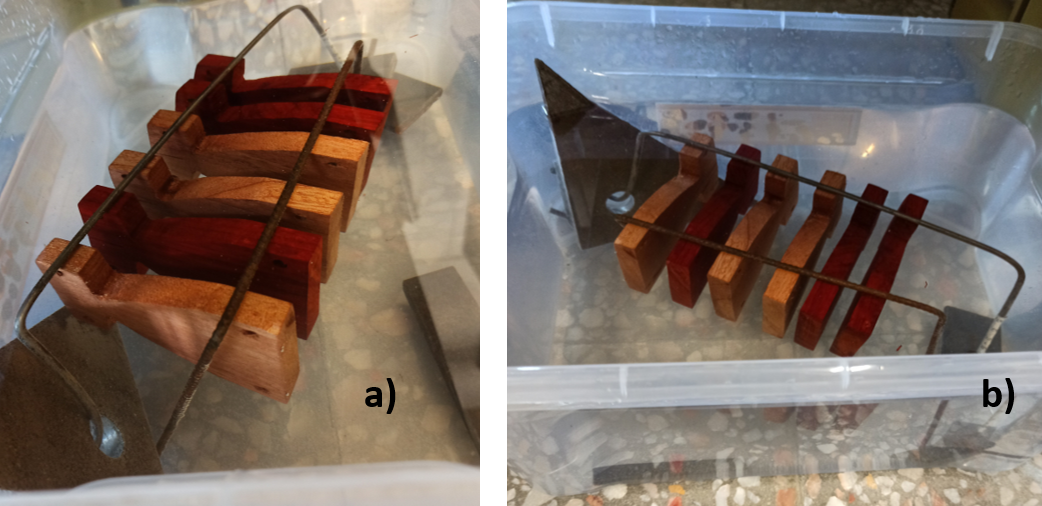
\includegraphics[width=\textwidth]{Figures/WaterSpecimens}
\decoRule
\caption[Specimen into water]{Specimens put into water in order to reach 30\% and 20\% Moisture Content in each specimens}
\label{fig:Fig13}
\end{figure}
The system was designed in order to prevent the specimens from rising to the surface by flotation. But also, to minimize the specimen surface in contact with the system. Indeed, it allows to maximize the MC rise which take less time to reach the desired MC levels. This fact was verified when all the specimens (from E2 and E3 experiment) were put together into water. Indeed, the system was not designed for 12 specimens, and the specimens were really closed. It involves a slower increase of the MC.

After XXXh for Experiment 1 specimens and XXXh for Experiment 2 specimens, specimens were weighed again. Thanks to these weights, it was possible to plot a shape about, how the MC decreases, and how the weight evolve compared to time. A quick look to the decrease of MC into Okoume specimens show that until 20\% MC, every hour almost 1\% MC is loose. From this value until the ambient MC, the MC decrease process becomes slower as it is shown on \ref{fig:Fig15_b}, with decreasment less than 0.4\% every hour.

Thanks to E3 daily weight, it appears that both species, Okoume and Padouck, earn a constant MC. The difference is the value of this constant increasing. Okoume specimens earn approximately 5\% MC each day while Padouck ones earn around 2\% MC


To test the specimens at the waited MC, plots as the \ref{fig:Fig15_a} were used. Indeed, by looking to there weight when they were out the water, a MC was obtained, and by looking to the difference between the current MC and the waited one can be given in term of hours. So it was possible to have an approximation of the time before doing the experiments.

Then, all the specimens were weighted to have an idea of the MC in each just before the test. They were dried again after being tested, due to the incertitud of the first drying process. It must be noticed that the MC value is not perfect due to many parameters as the loose of material after the crack, the scale incertitude...
The purpose of this work was to have an idea of the impact of MC on the crack propagation.

As visible on \ref{fig:Fig17} the charcteristic patern replace the grid from the grid method as used in \parencite{Reference7} or a markers tracking method like in \parencite{Reference18} work. The patern is different for every specimen. From the second sample tested, a scale was added on the specimens.
The precrack was measured again and more precisely with a calliper. The measure can change, due to the swelling of the wet specimens.

\textbf{\textit{\underline{Ajouter l'evolution du précrack proportionellemeent à l'augmentation detaille de l'éprouvette.
}}}
%----------------------------------------------------------------------------------------
%	SUBSECTION 2
%----------------------------------------------------------------------------------------
\section{Fracture test set-up}

The fracture tests were carry out using a universal testing machine. The first step was to asssembled the grips in the press. Then a displacement of 0.033mm/s was input in the press controler program. A 10kN load was also input to be sure that the displacement will occure correctly. Then the same load was applied but from the third specimen tested, a displacement of 0.015mm/s was finally applied. The final set up is shown on \ref{fig:Fig18}.

It was important to stop the press between two tests in order to avoid the overheating of the oil/water allimenting the hydraulic press.

\begin{figure}[t]
	\centering
	\includegraphics[scale=0.05,angle=-90]{Figures/SetUp}
	\decoRule
	\caption[Final setup]{Setup composed of the camera and it lense linked to MatchId, the green constant light, tripods, the hydraulic press and the specimen griped to it.}
	\label{fig:Fig18}
\end{figure}

The temperature and relative humidity during the test were controlled thanks to a sensor placed in the test room. The \ref{fig:Fig19} gives an idea of the conditions which were almost constant, even if the temperature increase with increase of the hydraulic press utilisation time.

\begin{figure}[t]
	\centering
	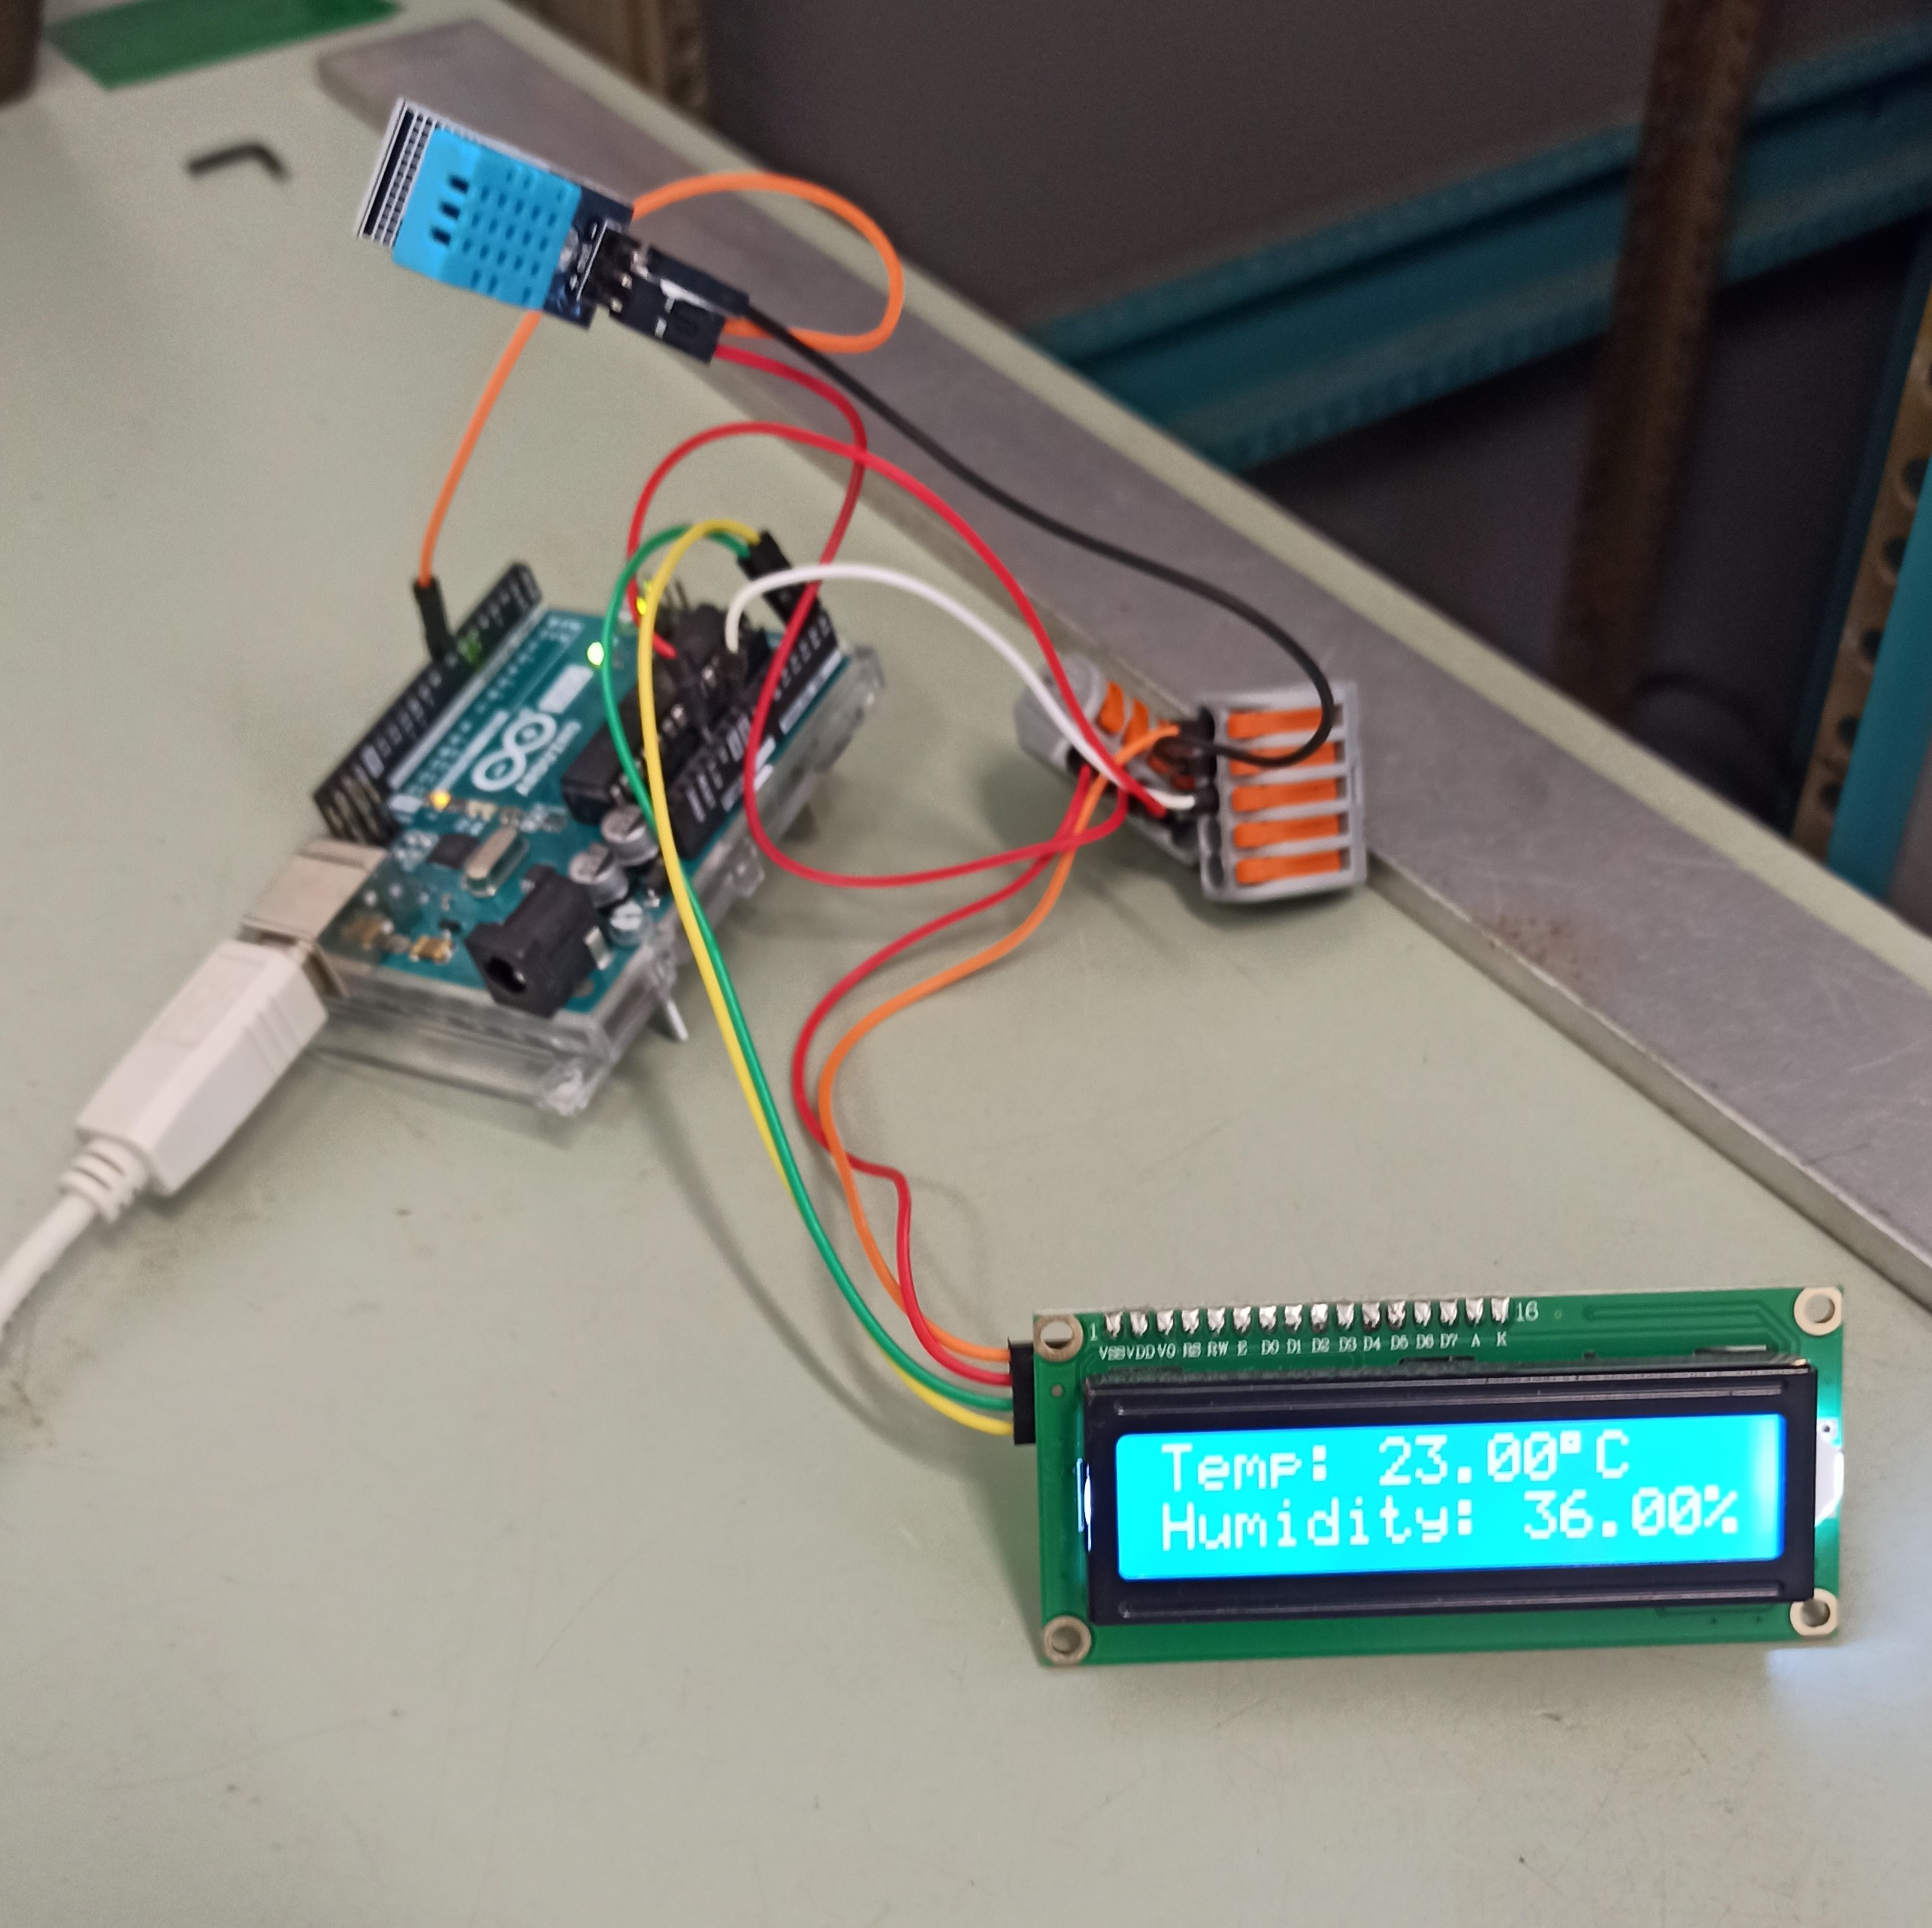
\includegraphics[scale=0.08]{Figures/Temperature_ relative_humidity}
	\decoRule
	\caption[Climatical conditions of the test]{Climatical conditions of the test in a closed room}
	\label{fig:Fig19}
\end{figure}

\section{Optical system set-up}

An Allied Vision Manta 505B 2/3'' camera coupled to an Opto Engineering TC 23 36 telecentric lens were used for image formation and acquisition. The camera is equiped with Charge-Coupled Device (CCD) sensor with pixel resolution of 2452 (H) $\times$ 2056 (V) (5MP) and sensor size of 2/3''. The monovision camera-lens optical system was fixed on a tripod and its spatial position oriented with regard to the target surface of interest. The telecentric lens has a magnification fator of \num{0.243}$\times$, allowed to image a field of view, in the object space, of 36.2$\times$27.1 \si{\milli\meter\squared}. The front of the lens was positioned at a working distance of 103.5 \si{\milli\meter} with an apperture of $f$/8, yielding a field of depth of 11 \si{\milli\meter}.

A high power adjustable ring light was used to illuminate the region of interest. A monochromatic version corresponding to a green wavelengths of \num{525} \si{\nano\meter} was used from which the highest spectral response of the camera sensor will be expected.

All the specimens were painted to obtain a speckle pattern suitable for image correlation. A thin layer of white paint was firstly added using a mate spray, followed by a diffuse distribution of black paint to create a unique local pattern across the region of interest at the crack tip (Figure~\ref{fig:Fig17}).

\begin{figure}[t]
	\centering
	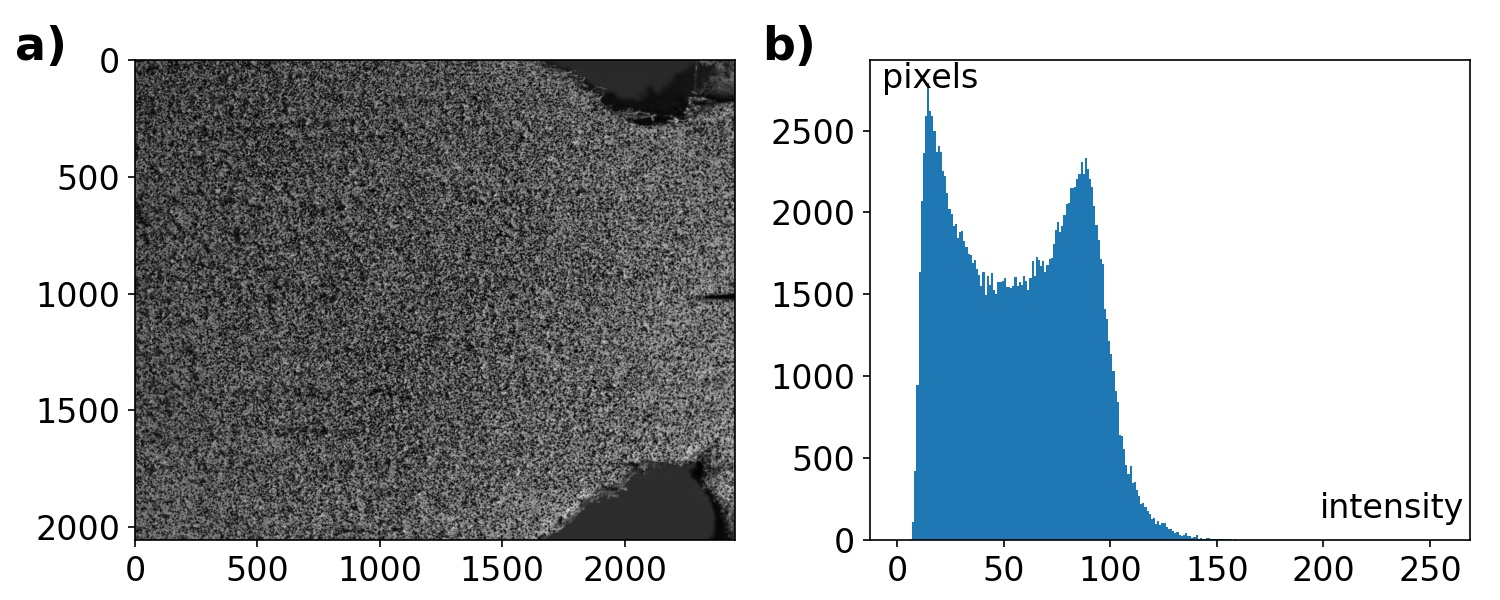
\includegraphics[width=.9\textwidth]{Figures/SpecklePattern}
	\decoRule
	\caption{(a) Speckle pattern typycally obtained for DIC measurements (2452 $\times$ 2056
	pixels\textsuperscript{2}); (b) Histogram
	of the
	speckle image
		(256
	gray levels, 8 bits camera).}
	\label{fig:Fig17}
\end{figure}

\section{DIC measurements and settings}

The DIC setting parameters can have a significant influence on the kinematic fields obtained by image correlation (\textit{e.g.} subset size, subset step, \ldots) and numerical differentiation (\textit{e.g.} strain windows size) algorithms \cite{Pereira2018}. These settings represent fundamental parameters since they will define the spatial resolution and accuracy associated to the DIC measurements, both in displacement and strain fields.  Therefoere, a parametric study was carried out to justify the DIC setting for the current
application, in a balance between resolution and spatial resolution. This study was carried ot in the Parametric Module of MatchID 2D software. Table~? defines the range of values defined in this performance analysis which includes the subset size ($f_s$), subset step, affine and quadratic displacement shape functions, the strain windows size and the order of the polynomial fitting function. The pre-selected range of values are deemed to be representative of the range of accepble DIC setting parameters. For instance, The lower pixel boundary is constrained by aliasing effects, which is a function of the speckle size on the imaged pattern. The subset size defines the target matching pattern used in the correlation algorithm. A rule of thumb will be three contrasted speckles per subset. The average speckle size was determined as 4.5 pixels. Therefore, the mininum subset step was set to 15 pixels. The upper pixel limit can be problem-dependent taking into account the deformation gradients expected within the region of interest, in a balance between spatial resolution and resolution. As a guideline, larger subsets improves the resolution but decreases spatial resolution. Parameters such as the subset step ($f_p$) (distance between centroids of adjacent subsets, units: pixels) and the strain window $\varepsilon_w$ (number of subsets central points used to define a mesh of data points over which a piecewise polynomial fitting will be applied, using least-square regression, for strain reconstruction) will define a strain spatial resolution ($\Delta \varepsilon$) and virtual strain gauge (VSG), respectively, according to the following relationships \cite{Lava2013576,Pereira2018566}: $\Delta \varepsilon = (\varepsilon_w-1)f_p + f_s$ and $\mbox{VSG} = (\varepsilon_w-1)f_p + 1$ (unit: pixel). For convenience, these parameters can be converted to physical units in the object space (\textit{e.g.} mm), by simple multiplication by the conversion factor of the optical imaging system. All these external DIC parameters, therefore, must be carefully selected in the current study.


A single pair of images, including a reference and deformed image at a force of about 100 N were selected to carry out this study. The obtained results are shown in Figure ?. In this plot the signal of interest, is plotted with regard to a measure of the strain spatial resolution given by the parameter Virtual Strain Gauge (VSG). Both the $y$ component of the displacement and $\varepsilon_{yy}$ component of strain are presented to support the DIC setting selection. Therefore


